\documentclass[a4paper,10pt]{report}
\usepackage[OT1]{fontenc} 
\usepackage{fullpage}
\usepackage[latin1]{inputenc}
\usepackage{bbold}
\usepackage{textcomp}
\usepackage{pstricks-add}
\usepackage{pst-plot}
\usepackage{graphicx}
\usepackage{amsmath}
\usepackage{amssymb}
\usepackage{theorem}
\usepackage{algorithm}
\usepackage{algorithmic}
\usepackage{titlesec}
\usepackage[french]{babel}
\usepackage{listings}

\definecolor{green}{rgb}{.4,.804,0}

\floatname{algorithm}{Algorithme}
\renewcommand{\algorithmicrequire}{\textbf{Entr\'{e}e(s)}}
\renewcommand{\algorithmicensure}{\textbf{Sortie(s)}}
\renewcommand{\algorithmicdo}{\textbf{faire}}
\renewcommand{\algorithmicendwhile}{\textbf{fin du tant que}}
\renewcommand{\algorithmicend}{\textbf{fin}}
\renewcommand{\algorithmicif}{\textbf{si}}
\renewcommand{\algorithmicendif}{\textbf{fin du si}}
\renewcommand{\algorithmicelse}{\textbf{sinon}}
\renewcommand{\algorithmicelsif}{\textbf{fin du sinon}}
\renewcommand{\algorithmicthen}{\textbf{alors}}
\renewcommand{\algorithmicfor}{\textbf{pour}}
\renewcommand{\algorithmicforall}{\textbf{pour tout}}
\renewcommand{\algorithmicto}{\textbf{\`{a}}}
\renewcommand{\algorithmicendfor}{\textbf{fin du pour}}
\renewcommand{\algorithmicdo}{\textbf{faire}}
\renewcommand{\algorithmicloop}{\textbf{boucler}}
\renewcommand{\algorithmicendloop}{\textbf{fin de la boucle}}
\renewcommand{\algorithmicrepeat}{\textbf{répéter}}
\renewcommand{\algorithmicuntil}{\textbf{jusqu’à}}
\renewcommand{\algorithmicprint}{\textbf{afficher}}

\theoremstyle{break}
\newtheorem{Def}{D\'{e}finition}
\newtheorem{Prop}{Proposition}
\newtheorem{Rem}{Remarque}
\newtheorem{Nota}{Notation}
\newtheorem{Dem}{Demonstration}

\lstset{language=caml}

% Title Page
\title{Compression d'images par ondelettes}
\author{Benjamin CATINAUD}
\date{Ann\'{e}e 2017-2018}

\makeglossary

\begin{document}
\maketitle

\begin{abstract}
  Nowadays, million of pictures are sent every minute. Consequently, we have to create algorithms to compress this data.
  To this end, several solutions exist. The most famous is perhaps the Fast Fourier Transform, use by scientists. 
  However, this transform take care of frequencies in a signal but doesn't take its chronology into account. 
  To adress this issue, I suggest to study the Wavelet Transform. This paper will detail basics of wavelet theory, 
  as well as algorithms to transform and rebuild pictures with wavelets and, finally, discuss their efficiency.
\end{abstract}

\newpage

\section*{Introduction}

  \paragraph{} Aujourd'hui o\`{u} des millions d'images sont envoy\'{e}es chaque minute, une m\'{e}thode pour compresser ces donn\'{e}es,
    situ\'{e}es \`{a} l'interface t\'{e}nue entre humain et machine et t\'{e}moignant des interactions humaines, est par cons\'{e}quent requise. 
    Cette m\'{e}thode devra optimiser rapidit\'{e}, homogen\'{e}it\'{e}, integrit\'{e} et coh\'{e}sion de ces informations.
    
  \paragraph{} Pour ce faire, plusieurs solutions peuvent \^{e}tre mises en place. Typiquement, les physiciens utilisent dans la plus grande
    majorit\'{e} des cas la transformation $FFT$ (pour Fast Fourier Transform).
	
  \paragraph{} Cependant, la transform\'{e}e de Fourier permet de bien distinguer les fr\'{e}quences d'un signal mais pas leur chronologie \cite{twt}.
    Cette particularit\'{e} peut \^{e}tre probl\'{e}matique dans certains cas lors de traitements du signal comme le cas de signaux non 
    sinuso\"{i}daux, notamment pour les images. Ainsi, nous choisirons de travailler avec la transformation par ondelettes,
    fonctions de carr\'{e} int\'{e}grable, \`{a} support compact et d'int\'{e}grale nulle.
    
  \paragraph{} La th\'{e}orie des ondelettes, mise au point dans les ann\'{e}es 1980 par plusieurs chercheurs dont notamment Yves Meyer
    et Jean Morlet, a connu ainsi un rapide succ\`{e}s que ce soit dans le traitement de signaux sismiques (domaine qui a initi\'{e}
    la recherche dans cette th\'{e}orie) ou dans le traitement des images.
      
      
  \paragraph{} Ce travail va donc s'appuyer sur la th\'{e}orie des ondelettes afin de r\'{e}pondre au probl\`{e}me de la compression
      d'images en utilisant \`{a} profit cette th\'{e}orie. Apr\`{e}s avoir donn\'{e} la d\'{e}finition d'une ondelette et avoir 
      d\'{e}fini l'analyse multir\'{e}solution, nous d\'{e}taillerons l'algorithme de la transformation par ondelettes 
      (abr\'{e}g\'{e} dans la suite l'algorithme $FWT$) con{\c c}u par St\'{e}phane Mallat. 
      Ensuite, nous discuterons de l'efficacit\'{e} de cet algorithme du point de vue de la complexit\'{e} ainsi que les pertes occasionn\'{e}es. \newline

\newpage

  \section{I. Une ondelette, c'est quoi ?}
    
    \begin{Def}[Ondelette m\`{e}re et ondelettes filles]
	$\phantom{Prop}$ Soit $\psi \; \in \; L^2(\mathbb{R},\mathbb{R})$ \`{a} support compact et telle que 
	      $ \int_{\mathbb{R}} \psi $ converge et vaut $ 0 $. \newline
	$\phantom{Prop}$ Soit $ (\psi_{j,k})_{ (j, k) \; \in \; \mathbb{Z}^2 } $ une famille de fonctions de $L^2(\mathbb{R},\mathbb{R})$ d\'{e}finie par : \newline
	$\phantom{Soit \psi \; \in \; L^2(R,R)}$ $ \forall (j, k) \; \in \; \mathbb{Z}^2, \forall x \; \in \; \mathbb{R}, 
	      \psi_{j,k}(x) \; = \; \frac{1}{\sqrt{2^j}} \psi (\frac{2^j x - k}{2^j})$ \newline
	$\phantom{Prop}$ On dit alors que $\psi$ est l'ondelette m\`{e}re \cite{twt} et que la famille $ (\psi_{j,k}) $ issue de translations et de dilatations
	    de l'ondelette m\`{e}re forme la famille des ondelettes filles.
    \end{Def}
	    
    \paragraph{Exemple} Ondelette de Haar \newline
	$\phantom{Prop}$ Soit $\psi$ la fonction d\'{e}finie par : $ \psi \; = \; \mathbb{1}_{[0;\frac{1}{2}[} \; - \; \mathbb{1}_{[\frac{1}{2};1[}$. \cite{comp} \newline
	$\phantom{Prop}$ $ \psi $ \'{e}tant constante par morceaux, $ \int_{\mathbb{R}} \psi $ converge et vaut $ 0 $. \newline
	$\phantom{Prop}$ De plus, son support est clairement compact. \newline
	$\phantom{Prop}$ La famille orthonormale associ\'{e}e \`{a} l'ondelette m\`{e}re $\psi$ est alors :
	\begin{center}
	  $ (\psi_{j, k})_{(j, k) \in \mathbb{Z}^2} $ o\`{u} 
	  $ \forall j, k \in \mathbb{Z}, \forall x \in \mathbb{R}, \psi_{j,k}(x) \, = \, \frac{1}{\sqrt{2^j}} \psi (\frac{x - 2^j k}{2^j}) $
	\end{center}
	
	\begin{figure}[!h]
	  \centering
	
	  \begin{pspicture}(-0.5,-1.5)(1.5,1.5)
	    \psset{algebraic=true}
	    \psset{xunit = 3cm, yunit = 1cm}
	    \psaxes{->}(0,0)(-0.5,-1.5)(1.5,1.5)
	    \psplot{0}{0.5}{1}
	    \psline[linestyle=dotted](0.5,1)(0.5,-1)
	    \psplot{0.5}{1}{-1}
	    \psline[linestyle=dotted](1,-1)(1,0)
	  \end{pspicture}
	  
	  \caption{Courbe repr\'{e}sentative de $\psi$}
	  
	\end{figure}
	
  \section{II. Analyse multir\'{e}solution}

      \begin{Def}[Espace d'approximation]
	  $\phantom{Prop}$ Soit $ j \in  \mathbb{Z} $. On appelle espace d'aproximation \`{a} l'\'{e}chelle $ 2 ^ j $
	  l'espace vectoriel des fonctions de $ L^2(\mathbb{R}, \mathbb{R}) $ constantes sur 
	  les intervalles de la forme $ [2^j k; 2^j (k \, + \, 1)[, \; k \; \in \; \mathbb{Z}$ \cite{comp}. On le note $ V_j $.
      \end{Def}
	      
      \begin{figure}[!h]
	\centering
	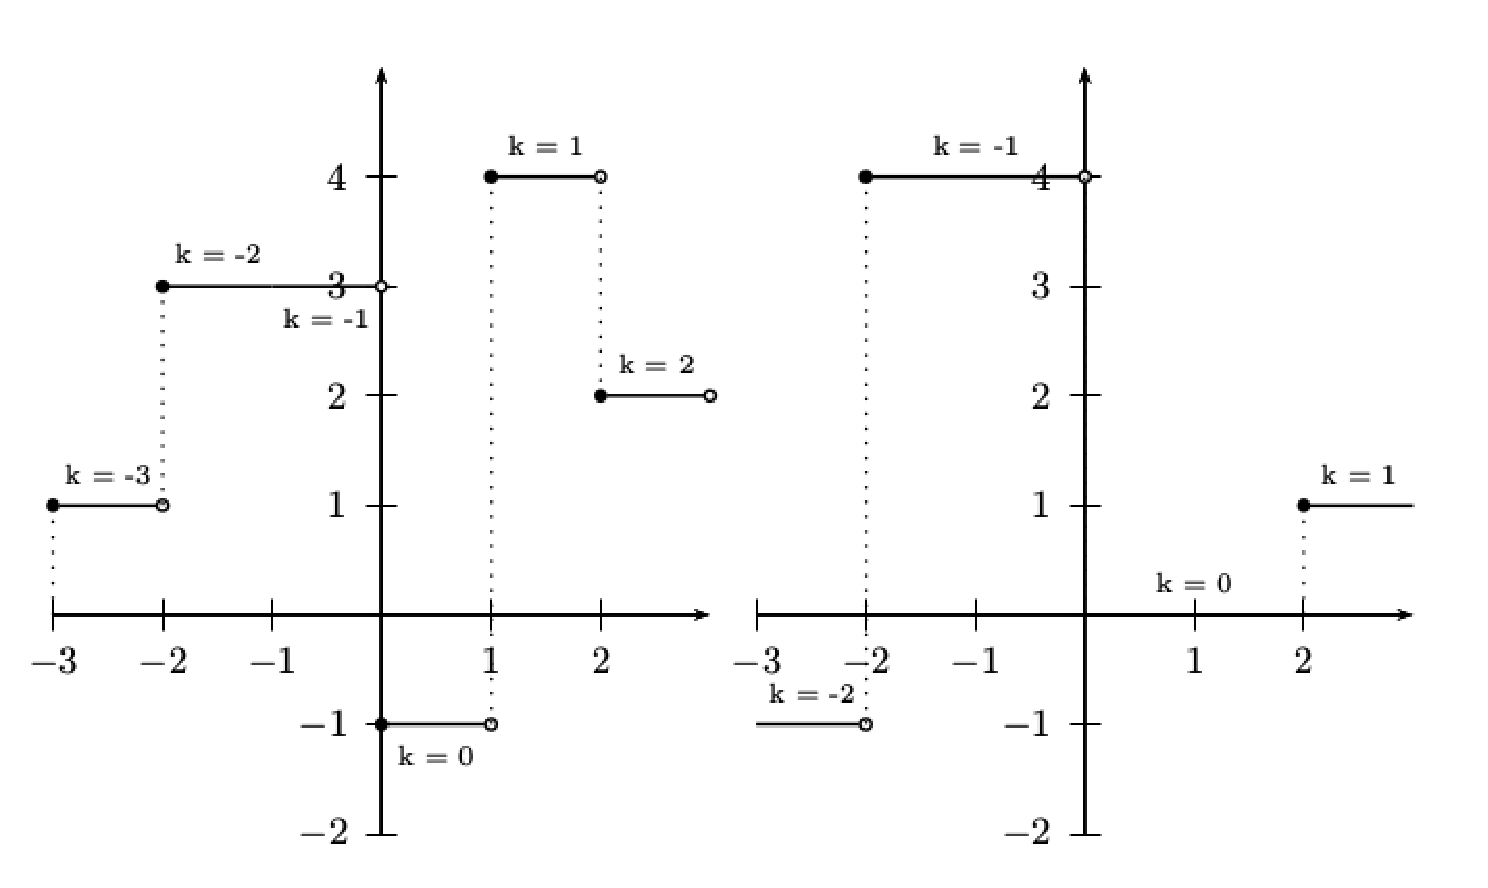
\includegraphics[width = 0.7 \linewidth]{espaces.eps}
	\caption{Exemple graphique d'une fonction de $V_0$ (\`{a} gauche) et de $V_1$ (\`{a} droite)}
      \end{figure}
      
\newpage
	      
      \begin{Prop}
	$\phantom{Prop}$ Les espaces $(V_j)_{j \in \mathbb{Z}}$ v\'{e}rifient les propri\'{e}t\'{e}s suivantes \cite{comp} :
	\begin{itemize}
	  \item[$(i)$] $ \forall j \in \mathbb{Z}, V_{j + 1} \subseteq V_j $
	  \item[$(ii)$] $ \displaystyle \bigcup_{j \in \mathbb{Z}} V_j $ est dense dans $ L^2(\mathbb{R}, \mathbb{R}) $
	\end{itemize}
      \end{Prop}
	  
    \begin{Prop}[Caract\'{e}risation des espaces d'approximation]
	  $\phantom{Prop}$ On a : 
	  
	  \begin{center}
	  $ \forall j \in \mathbb{Z}, V_j \; = \; 
	  \Bigg< \Big\{ \phi_{j,k} = \frac{1}{\sqrt{2^j}} \mathbb{1}_{[2^j k; 2^j (k \, + \, 1)[}, \; k \in \mathbb{Z} \Big\} \Bigg> $ 
	  \end{center}
	  
	  $\phantom{Prop}$ La famille $ (\phi_{j, k})_{(j, k) \in \mathbb{Z}^2} $ est ainsi une famille d'ondelettes filles issue de l'ondelette
	    m\`{e}re $ \phi \; = \; \mathbb{1}_{[0 ; 1[} $.
    \end{Prop}
	    
    \paragraph{} L'id\'{e}e de la transformation par ondelettes est ainsi de calculer les projections d'une fonction
	$ f \in L^2(\mathbb{R}, \mathbb{R}) $ sur les espaces $ V_j $ pour un $ j \in \mathbb{Z} $ donn\'{e}.
	Plus le $ j $ diminue, plus l'approximation ainsi faite est pr\'{e}cise.
	
    \begin{Def}[Espace des d\'{e}tails]
	$\phantom{Prop}$ On d\'{e}finit la notion d'espace de d\'{e}tails $ W_j , $ pour $ j \, \in \, \mathbb{Z} $, tel que \newline
	$ V_{j - 1} \, = \, V_j \displaystyle \bigoplus^\perp W_j $ \newline
	Ainsi, par d\'{e}finition, la connaissance de $ W_j $ et $ V_j $ permettent d'obtenir $ V_{j - 1} $.
    \end{Def}
    
    \begin{Prop}[Caract\'{e}risation des espaces de d\'{e}tails]
	  $\phantom{Prop}$ On a : 
	  
	  \begin{center}
	  $ \forall j \in \mathbb{Z}, W_j \; = \; 
	  \Bigg< \Big\{ \psi_{j,k} \; = \; \frac{1}{\sqrt{2^j}} (\mathbb{1}_{[2^{j - 1} k ; 2^{j - 1} (k + 1)[} - 
		\mathbb{1}_{[2^{j - 1} (k + 1) ; 2^{j - 1} (k + 2)[} ),  \; k \in \mathbb{Z} \Big\} \Bigg> $ 
	  \end{center}
    \end{Prop}

    \begin{Rem} On remarque une relation de r\'{e}currence entre les ondelettes $ \psi_{j,k} $ et $ \phi_{j,k} $ pour tout $ k, j \in \mathbb{Z} $ :
	\begin{center}
	  $ \phi_{j,k} = \frac{1}{\sqrt{2}} (\phi_{j - 1, 2 k} + \phi_{j - 1, 2 k + 1}) $ \\
	  $ \psi_{j,k} = \frac{1}{\sqrt{2}} (\phi_{j - 1, 2 k} - \phi_{j - 1, 2 k + 1}) $
	\end{center}
    \end{Rem}
    
    \paragraph{} Cette remarque nous am\`{e}ne ainsi \`{a} l'algorithme de Mallat qui permet la transformation par ondelettes d'une image.
      
\newpage
	
  \section{III. Algorithme de transformation par ondelettes ou Algorithme de Mallat}

    \paragraph{} Dans toute la suite, pour illustrer les propos, nous utiliserons l'image suivante
	\begin{figure}[!h]
	    \centering
	    
	    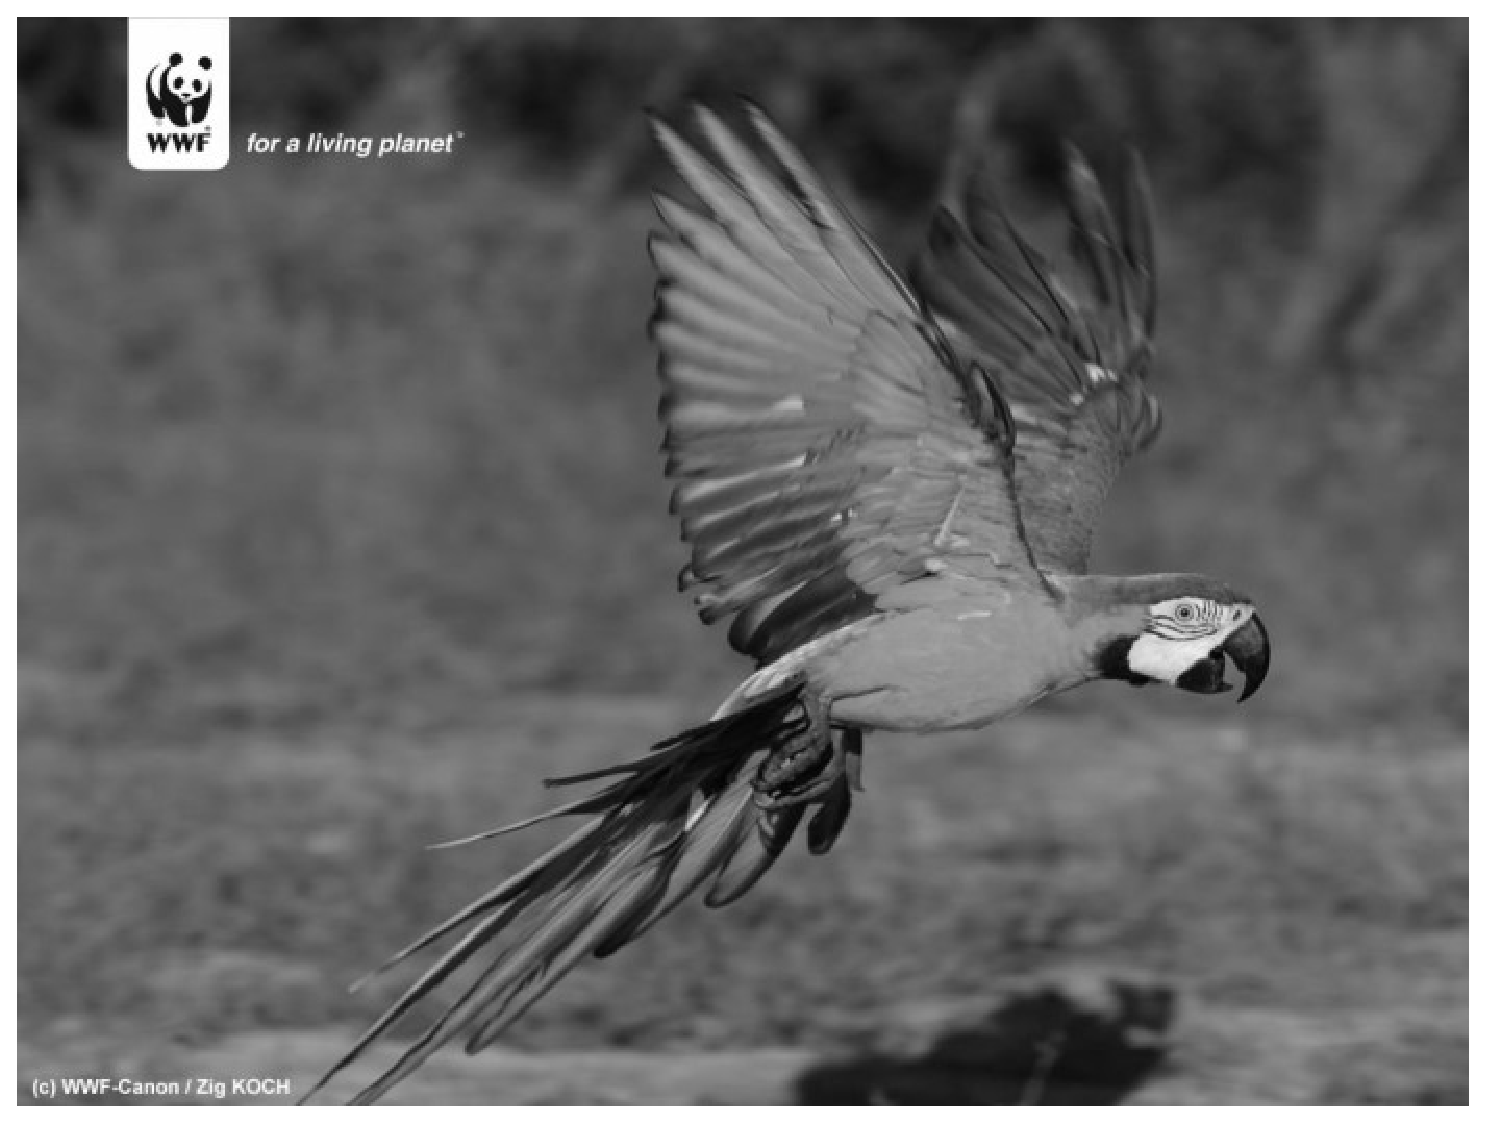
\includegraphics[width = 0.4 \linewidth]{ara_orig.eps}
	    
	    \caption{Image originale}
	\end{figure}
	
    \begin{Def}[Vecteurs associ\'{e}s \`{a} la transformation par ondelettes de Haar]
      $\phantom{Prop}$ D'apr\`{e}s la remarque pr\'{e}c\'{e}dente, on pose les vecteurs associ\'{e}s \`{a} 
      la transformation par ondelettes de Haar suivants :
      \begin{center}
	$ \mathcal{H}_a \; = \; \frac{1}{2} (1, 1) \; \in \; \mathbb{R}^2 $ pour les espaces $(V_j)_{j \in \mathbb{Z}}$ \\
	$ \mathcal{H}_d \; = \; \frac{1}{2} (1, -1) \; \in \; \mathbb{R}^2 $ pour les espaces $(W_j)_{j \in \mathbb{Z}}$
      \end{center}
    \end{Def}
	
    \begin{Def}[Fonction filtre]
	$\phantom{Prop}$ Soit $ n \in \mathbb{N} $. Soient $ b, x \in \mathbb{R}^n $. Soit $ a \in \mathbb{R}^* $. \newline
	$\phantom{Prop}$ On d\'{e}finit un nouveau vecteur $ y \in \mathbb{R}^n $, image de $x$ par la fonction $ \Phi_{a,b} $ tel que :
	\begin{center}
	  $ \forall i \in [1;n], \; y_k \; = \; \frac{1}{a} \displaystyle\sum_{i = 1}^k b_i x_{k - i} $
	\end{center}
	$\phantom{Prop}$ On notera $\varPhi$ la fonction filtre sur les espaces d'approximation
	et $\varPsi$ celle sur les espaces de d\'{e}tails
    \end{Def}
	
    \paragraph{} Avant d'\'{e}tudier l'algorithme, il reste encore \`{a} d\'{e}finir une fonction permettant d'extraire un sous vecteur.
    
    \begin{Def}[Fonction d'\'{e}chantillonage]
	$\phantom{Prop}$ On note $\downarrow_k $, pour $k \in [1;n]$ la fonction suivante :
	\begin{center}
	  $ \downarrow_k \, : \mathbb{R}^n \longrightarrow \mathbb{R}^{\lfloor n / k \rfloor} $ \\
	  $ (x_1, x_2, ..., x_n) \longmapsto (x_k, x_{2 k}, ..., x_{\lfloor n / k \rfloor k}) $
	\end{center}
    \end{Def}
      
\newpage

    \paragraph{Algorithme de Mallat} Consid\'{e}rons une image sous forme de matrice $M \in M_{n,m}(\mathbb{R})$, o\`{u} l'on supposera
	que $n$ et $m$ sont deux multiples d'une puissance de $2$, quitte \`{a} la normaliser en ajoutant des z\'{e}ros. \newline
	
	Pour calculer $V_{-j}$ et $W_{-j}$, on applique la fonction filtre en premier lieu sur les lignes de $M$. \newline
	On applique alors les fonctions $ \varPhi $ et $\varPsi$ au vecteur 
	$ M_{i,[1;m/2^j]} \; = \; (M_{i,1}, M_{i,2}, ..., M_{i, m/2^j}) $ 
	puis on applique au r\'{e}sultat ainsi obtenu la fonction de sous-\'{e}chantillonage $\downarrow_2$.
	En deuxi\`{e}me lieu, on applique aux colonnes not\'{e}es $M_{[1;n/2^j], j}$ de cette nouvelle matrice ces m\^{e}mes fonctions.
	
	L'algorithme, pouvant \^{e}tre consid\'{e}r\'{e} comme une fonction not\'{e}e $TW$, 
	pour calculer la transform\'{e}e par ondelettes sur les espaces $V_{-j_V}$ et $W_{-j_V}$ est donc le suivant :
	
	\begin{algorithm}
	  \caption{Transform\'{e}e par ondelettes d'une matrice}
	  
	  \begin{algorithmic}
	    \REQUIRE { une matrice $M \in M_{n,m}(\mathbb{R}) $ et un entier $j_V \in \mathbb{N}$ }
	    \IF {$n$ ne divise pas $2^{j_V}$ } 
	      \STATE {Ajouter $(n \, - \, n \, \% \, 2^{j_V})$ lignes de z\'{e}ros \`{a} $M$} 
	    \ENDIF
	    \IF {$m$ ne divise pas $2^{j_V}$ } 
	      \STATE {Ajouter $(m \, - \, m \, \% \, 2^{j_V})$ colonnes de z\'{e}ros \`{a} $M$} 
	    \ENDIF
	    
	    \FOR { $k = 0$ \TO $j_V - 1$}
	      \FOR { $i = 1$ \TO $n / 2^k$}
		\STATE { Affecter au vecteur $M_{i,[1;\frac{m}{2^{k + 1}}]}$ le r\'{e}sultat de
		  la fonction $ (\downarrow_2 \, $o$ \, \varPhi) $ appliqu\'{e} au vecteur $M_{i,[1;\frac{m}{2^k}]}$ }
		\STATE { Affecter au vecteur $M_{i,[\frac{m}{2^{k + 1}} + 1;\frac{m}{2^k}]}$ le r\'{e}sultat de
		  la fonction $ (\downarrow_2 \, $o$ \, \varPsi) $ appliqu\'{e} au vecteur $M_{i,[1;\frac{m}{2^k}]}$  }
	      \ENDFOR
	      \FOR { $j = 1$ \TO $m / 2^k$}
		\STATE { Affecter au vecteur $M_{[1;\frac{n}{2^{k + 1}}],j}$ le r\'{e}sultat de
		  la fonction $ (\downarrow_2 \, $o$ \, \varPhi) $ appliqu\'{e} au vecteur $M_{[1;\frac{n}{2^k}],j}$ }
		\STATE { Affecter au vecteur $M_{[\frac{n}{2^{k + 1}} + 1;\frac{n}{2^k}],j}$ le r\'{e}sultat de
		  la fonction $ (\downarrow_2 \, $o$ \, \varPsi) $ appliqu\'{e} au vecteur $M_{[1;\frac{n}{2^k}],j}$  }
	      \ENDFOR
	    \ENDFOR
	    \ENSURE {La matrice $M$ ainsi obtenue}
	  \end{algorithmic}

	\end{algorithm}

	Avec l'image t\'{e}moin, on obtient l'image suivante pour $V_{-1}$ i.e. $j_V \, = \, 2$:
	\begin{figure}[!h]
	    \centering
	    
	    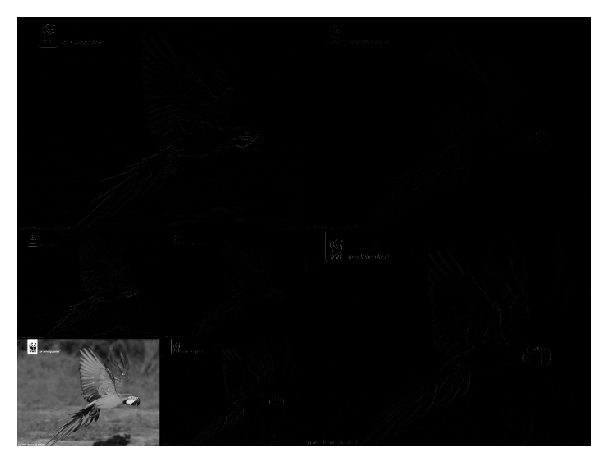
\includegraphics[width = 0.4 \linewidth]{ara_wt_V1.eps}
	    
	    \caption{Transform\'{e}e par ondelettes de l'image t\'{e}moin pour $j_V \, = \, 2$}
	\end{figure}
      
\newpage

    \paragraph{} D'apr\`{e}s la d\'{e}finition 3, comme $ \forall j \in \mathbb{Z}, V_{j - 1} \, = \, V_j \displaystyle \bigoplus^\perp W_j $, on en 
	d\'{e}duit l'algorithme de reconstruction suivant :
    
    \begin{algorithm}
      \caption{Reconstruction d'une matrice}
      
      \begin{algorithmic}
	\REQUIRE { une matrice $M \in M_{n,m}(\mathbb{R}) $ et un entier $j_V \in \mathbb{N}$ }	
	\FOR { $k = j_V - 1$ \TO $0$}
	  \FOR { $j = 1$ \TO $m / 2^k$}
	    \STATE { Affecter au vecteur $M_{[1;\frac{n}{2^k}],j}$  la somme du r\'{e}sultat de la fonction 
		$ (\varGamma \, $o$ \, \uparrow_2) $ appliqu\'{e}e au vecteur $M_{[1;\frac{n}{2^{k + 1}}],j}$ 
		et du r\'{e}sultat de la fonction $ (\varOmega \, $o$ \, \uparrow_2) $ appliqu\'{e}e au vecteur
		$M_{[\frac{n}{2^{k + 1}} + 1;\frac{n}{2^k}],j}$ }
	  \ENDFOR
	  \FOR { $i = 1$ \TO $n / 2^k$}
	    \STATE { Affecter au vecteur $M_{i,[1;\frac{m}{2^{k}}]}$  la somme du r\'{e}sultat de la fonction 
		$ (\varGamma \, $o$ \, \uparrow_2) $ appliqu\'{e}e au vecteur $M_{i,[1;\frac{m}{2^{k + 1}}]}$ 
		et du r\'{e}sultat de la fonction $ (\varOmega \, $o$ \, \uparrow_2) $ appliqu\'{e}e au vecteur
		$M_{i,[\frac{m}{2^{k + 1}} + 1;\frac{m}{2^k}]}$  }
	  \ENDFOR
	\ENDFOR
	\ENSURE {La matrice $M$ ainsi obtenue}
      \end{algorithmic}

    \end{algorithm}

 
\section*{IV. Un algorithme efficace ?}

  \subsection*{1) \'{E}tude de la complexit\'{e}}
    
    \begin{Prop}[Complexit\'{e} de la fonction $TW$]
      $\phantom{Prop}$ Soit $j_V \in \mathbb{N}$. Pour une image de taille $n$x$m$ pixels, la complexit\'{e} de $TW_{j_V}$ est :
      \begin{center}
	$ \boxed{O \Big(nm + n m^2 + m n^2 \Big)} $
      \end{center}

    \end{Prop}
    
    \begin{Rem}
      $\phantom{Prop}$ En utilisant les r\'{e}sultats des propri\'{e}t\'{e}s $8$ et $9$ on peut modifier la fonction $filter$ 
      pour faire chuter cette complexit\'{e} \`{a} $ O(nm) $. Cependant cette modification serait valable uniquement pour les
      ondelettes de Haar.
    \end{Rem}

    \paragraph{} Voici quelques performances en temps de l'algorithme $TW_{j_V}$ pour des matrices carr\'{e}es 
      (l'image d'origine est la m\^{e}me, seule diff\`{e}re la taille). 
      Les calculs se sont fait avec la configuration suivante :
      \begin{itemize}
       \item[-] CPU : Intel Code 2 CPU 2.40 GHz
       \item[-] RAM : 3.6 Go
      \end{itemize}

\newpage
    
    \begin{figure}[!h]
	\centering
	
	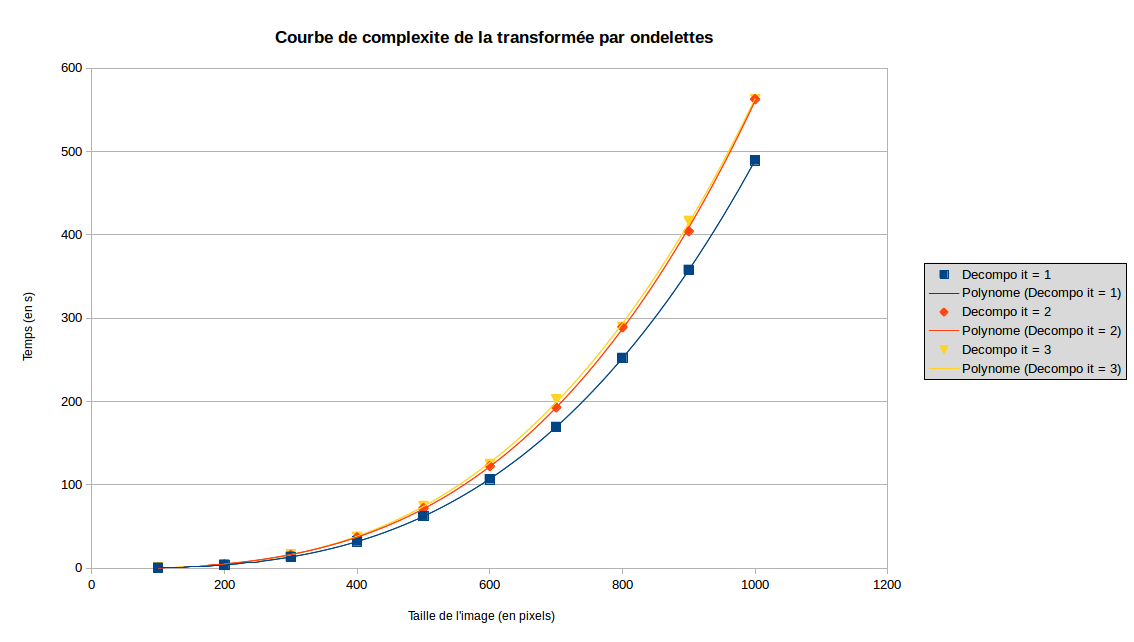
\includegraphics[width = 0.9 \linewidth]{complexite_decompo.eps}
	
	\caption{Complexit\'{e} de la fonction $TW_{j_V}$ en fonction de la taille de la matrice }
    \end{figure}

  \subsection*{2) Taux de compression}
  
    \begin{Nota}[Nombre d'octets d'une image]
      $\phantom{Prop}$ On notera dans la suite $No$ la fonction qui renvoie le nombre d'octets d'une image.
    \end{Nota}
    
    \begin{Def}[Fonction de compression]
      $\phantom{Prop}$ Ainsi on d\'{e}finit la fonction de compression pour $j_V \in \mathbb{N}$ comme mentionn\'{e} ci-dessus :
      \begin{center}
	$ \gamma_{j_V} : M_{n, m}(\mathbb{R}) \longrightarrow M_{n / 2^{j_V + 1}, m / 2^{j_V + 1}}(\mathbb{R}) $
      \end{center}
      $\phantom{Prop}$ O\`{u} les entiers $n$ et $m$ sont suppos\'{e}s \^{e}tre des puissances de $2$.
    \end{Def}
  
    \begin{Def}[Taux de compression]
      $\phantom{Prop}$ Soit $j_V \in \mathbb{N}$. On d\'{e}finit alors la fonction taux de compression not\'{e}e $\tau_C$ tel que :
      
      \begin{center}
	$ \tau_C :  M_{n,m}(\mathbb{R}) \longrightarrow [0;1] $ \\
	$ e \longmapsto \frac{No(\gamma_{j_V}(e))}{No(e)} $
      \end{center}

    \end{Def}
    
\newpage
    
    \paragraph{} Ainsi, on peut tracer le graphique suivant repr\'{e}sentant le taux de compression $\tau_C$ 
	o\`{u} $it$ repr\'{e}sente l'entier $j_V$. Les images utilis\'{e}es sont carr\'{e}es.

    \begin{figure}[!h]
	\centering
	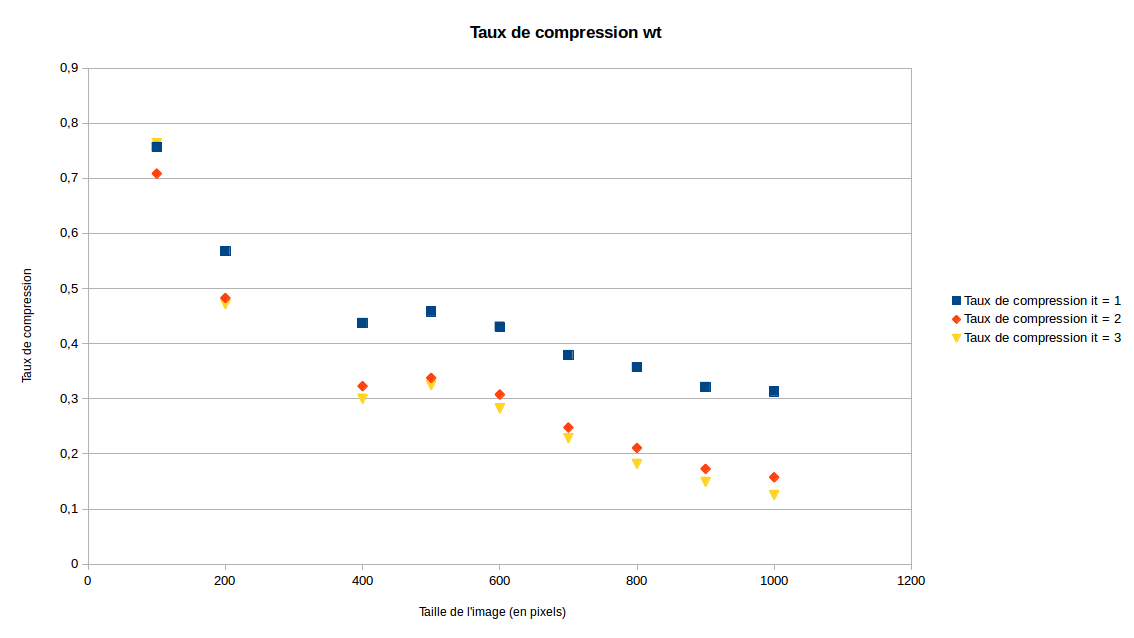
\includegraphics[width = 0.9 \linewidth]{taux_compression.eps}
	\caption{Taux de compression $\tau_C$ en fonction de la taille de la matrice}
    \end{figure}
    
    \begin{Rem}
      $\phantom{Prop}$ Ainsi, d'apr\`{e}s ce graphique, m\^{e}me si le temps requis est long, la compression semble plus efficace 
	pour les grandes images que pour les petites. De plus, plus $j_V$ augmente, plus la compression est efficace (en effet,
	on divise \`{a} chaque fois la taille de l'image par 2).
    \end{Rem}

    
  \subsection*{3) Estimation de l'erreur}
  
    \paragraph{} Comme on l'a vu dans la partie pr\'{e}c\'{e}dente, la fonction $\gamma$ introduit une erreur qui provient du fait 
	du passage d'une matrice de type $float$ au type $int$. De plus, l'appel \`{a} la fonction $Pixel\_matrix.intmatrix\_of\_matrix$
	introduit une autre erreur qui est le passage d'un intervalle de $\mathbb{R}$ \`{a} l'ensemble $[0;255]$.
	
    \paragraph{} On va donc introduire une fonction erreur. Pour cela, l'id\'{e}e la plus simple est d'utiliser une fonction distance.
	Cette fonction distance devra respecter deux crit\`{e}res :
	\begin{itemize}
	 \item [-] prendre en compte la taille de la matrice
	 \item [-] prendre en compte tous les \'{e}carts relatifs entre les coefficients
	\end{itemize}
    
\newpage
	
    \begin{Prop}[Distance de compression]
      $\phantom{Prop}$ On d\'{e}finit par cons\'{e}quent la distance suivante :
      \begin{center}
	$d : M_{n,m}(\mathbb{R}) \, $x$ \, M_{n,m}(\mathbb{R}) \longrightarrow \mathbb{R}^+ $ \\
	$ (M, N) \longmapsto \frac{\parallel M - N \parallel}{n m} $
      \end{center}

    \end{Prop}

    \begin{Def}[Fonction erreur]
      $\phantom{Prop}$ Soit $j_V \in \mathbb{N}$. On d\'{e}finit la fonction erreur comme suit avec $\gamma_{j_V}$ la fonction de compression 
	    et $\rho_{j_V}$ la fonction de d\'{e}compression :
      \begin{center}
	$\mathcal{E}_{j_V} : M_{n,m}(\mathbb{R}) \longrightarrow \mathbb{R}  $ \\
	$M \longmapsto d \Bigg(M, \Big(\rho_{j_V} \, $o$ \, \gamma_{j_V}\Big)(M) \Bigg)$
      \end{center}

    \end{Def}
    
    \paragraph{} En reprenant l'image originale, on obtient alors :

      \begin{figure}[!h]

	\begin{tabular}{cc}
	
	  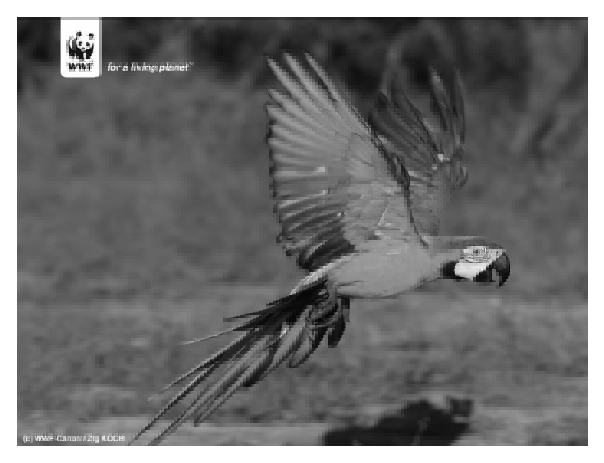
\includegraphics[width = 0.5 \linewidth]{decomp_ara.eps} &
	  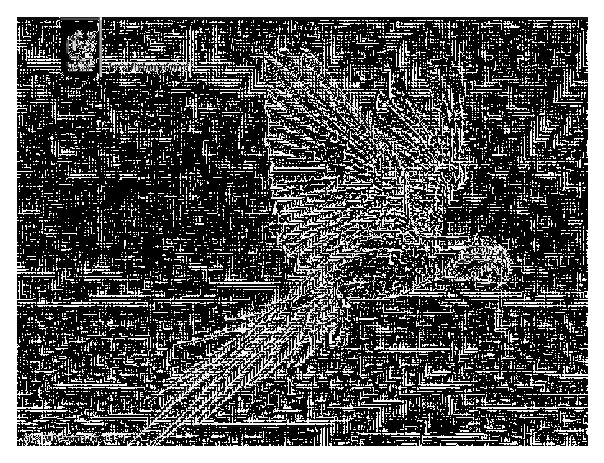
\includegraphics[width = 0.5 \linewidth]{error_ara.eps} \\	
	  
	\end{tabular}
	
	\caption{Image d\'{e}compress\'{e}e issue de $\Big(\rho_{j_V} \, $o$ \, \gamma_{j_V}\Big)$ (\`{a} gauche) et
	    image repr\'{e}sentant l'erreur commise (\`{a} droite)}
	
      \end{figure}

\newpage

\section*{Conclusion}

  \paragraph{} Ainsi, l'algorithme de Mallat permet de transformer une image par ondelettes. Lorsque cette transformation est faite,
      comme le poids de l'image ne change pas, il a \'{e}t\'{e} n\'{e}cessaire de trouver une solution afin de pouvoir effectivement
      compresser une image. Cette solution produit deux fichiers, ainsi n\'{e}cessaire lors de la transmission de ces donn\'{e}es.
      
  \paragraph{} On a \'{e}galement vu que l'algorithme de Mallat n'introduit pas d'erreur, c'est uniquement d\^{u} \`{a} la conversion
      d'une matrice de type $float$ au type $int$ que l'erreur est introduite. De plus, cette erreur diminue lorsque la taille de l'image
      augmente. Tout comme le taux de compression. Cependant, la complexit\'{e} temporelle est un s\'{e}rieux frein, m\^{e}me si une 
      complexit\'{e} de l'ordre de $O(n^3)$ est acceptable pour un algorithme travaillant sur les matrices. En effet, la transformation
      requiert la plupart des coefficients de la matrice et la fonction $filter$ s'effectue en temps quadratique (que l'on pourrait
      diminuer en un temps lin\'{e}aire dans le cas de l'ondelette de Haar). En titre de comparaison, la complexit\'{e} du produit matriciel
      na\"{i}f (c'est \`{a} dire, l'algorithme issue de la d\'{e}finition) a une complexit\'{e} de $O(n^3)$.
      
  \paragraph{} Enfin, lorsque l'on augmente le nombre d'it\'{e}rations de l'algorithme de Mallat (i.e. le nombre $j_V$),
      le taux de compression augmente mais l'erreur \'{e}galement. Il est donc peut \^{e}tre profitable de rester dans des petites
      valeurs de $j_V$ afin de garder l'int\'{e}grit\'{e} et la coh\'{e}sion des images.
      
  \paragraph{} Par cons\'{e}quent, l'algorithme propos\'{e} ici est plus efficace pour les grandes images plut\^{o}t que les petites, 
      m\^{e}me si l'algorithme s'effectue dans un temps plus long. Il faut donc trouver un compromis pour chaque taille d'image.
      Cependant, les probl\'{e}matiques actuelles de compression concernent surtout les grandes images et non les petites.

\newpage

  \begin{thebibliography}{1}
    \bibitem{comp}
      Pascal \textsc{Szacherski},
      \emph{Compression, ondelettes et algorithmes aff\'{e}rents},
      Janvier 2008
      
    \bibitem{ond}
      Phillip \textsc{K. Poon},
      \emph{Wavelets},
      College of Optical Sciences, University of Arizona,
      2012
      
    \bibitem{matlab}
      Philippe \textsc{Carr\'{e}} et R\'{e}mi \textsc{Cornillet},
      \emph{Code Matlab},
      respectivements professeur de l'universit\'{e} de Poitiers et responsable de l'\'{e}quipe Icones,
      \'{e}tudiant \`{a} l'\'{E}cole Normale Sup\'{e}rieure de Rennes

    \bibitem{twt}
      Ren\'{e} Alt,
      \emph{La transformation en ondelettes},
      Professeur \`{a} l'universit\'{e} Pierre et Marie Curie
    
    \bibitem{ond2}
      Olivier Rioul,
      \emph{Ondelettes r\'{e}guli\`{e}res: application \'{a} la compression d'images fixes},
      T\'{e}l\'{e}com ParisTech, 1993
      
    \bibitem{bmp}
      Marc Lorenzi,
      \emph{Code pour les images bmp},
      Professeur au lyc\'{e}e Camille Gu\'{e}rin
  \end{thebibliography}


\appendix

\chapter{}

  \begin{figure}[!h]
      \centering
      
      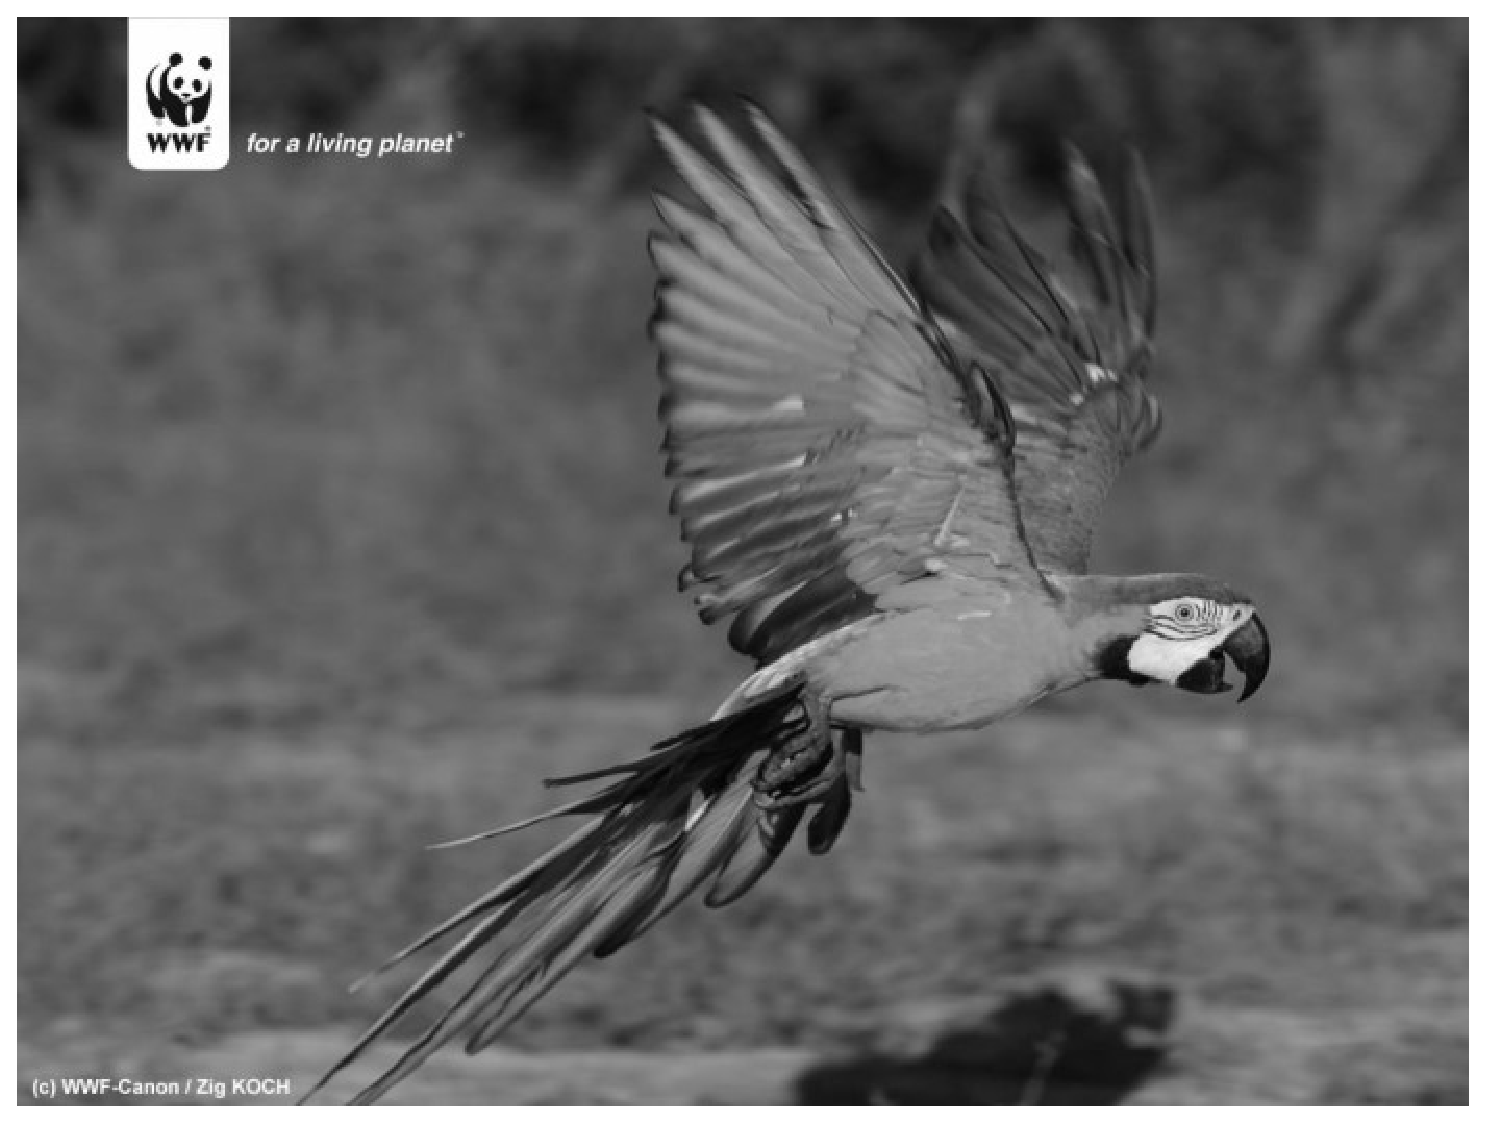
\includegraphics[width = 0.5 \linewidth]{ara_orig.eps}
      
      \caption{Image originale}
  \end{figure}

  \begin{figure}[!h]

    \begin{tabular}{cc}
    
      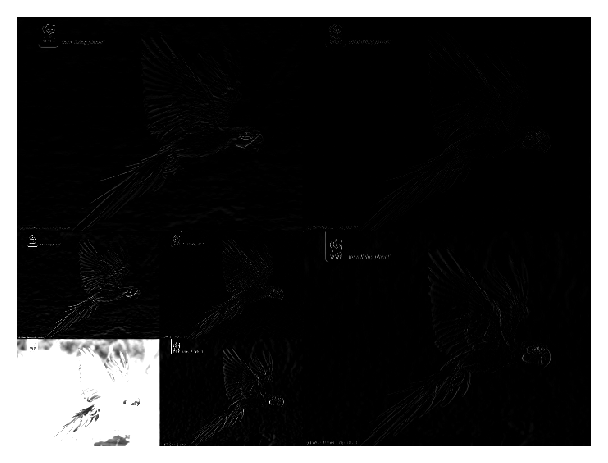
\includegraphics[width = 0.5 \linewidth]{ara_sqrt2.eps} &
      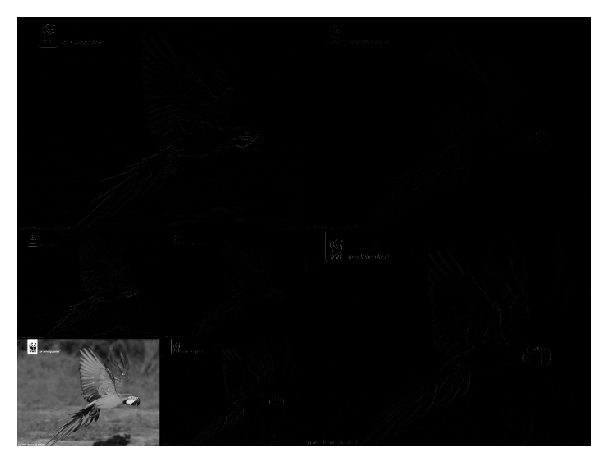
\includegraphics[width = 0.5 \linewidth]{ara_wt_V1.eps} \\	
      
    \end{tabular}
    
    \caption{Exemple de la diff\'{e}rence entre le choix du scalaire $\frac{1}{\sqrt{2}}$ (\`{a} gauche) 
	et du scalaire $\frac{1}{2}$ (\`{a} droite)}
    
  \end{figure}
  
  \paragraph{} On voit ainsi tr\`{e}s clairement que le scalaire $\frac{1}{2}$ permet de garder une bonne luminosit\'{e} de l'image originale.

\end{document}